% !TEX encoding = UTF-8
% !TEX TS-program = pdflatex
% !TEX root = ../tesi.tex
% !TEX spellcheck = it-IT

%************************************************



Il \emph{Micro-blogging} è un nuovo mezzo di comunicazione che permette agli utenti di pubblicare in broadcast  costantemente e in  "real time" brevi contenuti digitali, come testo, link, immagini o video. 
Questi contenuti vengono pubblicati in una rete sociale, in cui ogni utente può generare nuove informazioni, aggiornare informazioni esistenti e condividere o commentare informazioni pubblicate da altri utenti \cite{Java:2007:WWT:1348549.1348556}.  

Negli ultimi anni, questo mezzo di comunicazione ha attirato l'attenzione di una vasta  comunità  di ricercatori e aziende che operano in diversi ambiti.
La popolarità crescente di questi servizi di micro-blogging è dovuta alla loro portabilità, immediatezza e facilità d'uso. Queste caratteristiche consentono agli utenti di interagire istantaneamente e diffondere informazioni.

Virtualmente qualsiasi persona che assiste o è coinvolta in un qualsiasi evento è capace, grazie a questi micro-blog, di diffondere informazioni durante l'accaduto stesso. Ad esempio, durante i recenti conflitti, crisi sociali e manifestazioni\footnote{e.g.: primavera araba, proteste iraniane del 2009, elezioni presidenziali, etc.}, milioni di persone hanno utilizzato sistemi di micro-blogging come Twitter sia per diffondere notizie che per ricevere aggiornamenti sugli ultimi accadimenti.

Twitter è ad oggi il servizio di micro-blogging più utilizzato in assoluto. Con circa 284 milioni di utenti attivi al mese, ogni giorno vengono prodotti oltre 500 milioni di tweets al giorno. Gli utenti di Twitter, possono inviare in broadcast brevi status (\emph{tweets}), non  più lunghi di 140 caratteri,
 ad una rete di utenti (\emph{follower}) attraverso diversi dispositivi (e.g. smartphones, web-app, email, etc.).
 
Se da un lato la dimensionalità dei tweet rappresenta per alcuni utenti un forte limite, dall'altro rappresenta una delle caratteristiche fondamentali di Twitter: \emph{l'immediatezza}. Questo vincolo costringe gli utenti a produrre messaggi molto sintetici, quasi come slogan, che quindi sono più facili da diffondere.

%Inoltre, sebbene  i tweet siano caratterizzati da un contenuto molto ristretto, bisogna considerare che milioni di persone  \emph{twittano}\footnote{http://www.garzantilinguistica.it/ricerca/?q=twittare}  da ogni parte del mondo, a proposito di argomenti più disparati da manifestazioni sportive a crisi globali.
Monitorare e analizzare questo flusso di  contenuti generati degli utenti può portare a scoprire informazioni molto utili. Per esempio, molte aziende utilizzano Twitter sia per pubblicizzare e raccomandare i loro prodotti, che comprendere  le opinioni dei loro clienti riguardo i loro prodotti (o dei loro competitor) .
Inoltre i tweet sono stati analizzati per predire i risultati delle votazioni presidenziali, crimini \cite{Wang2012}, attività terroristiche o eventi. In generale, un evento può essere definito \emph{qualcosa che accade in un luogo e tempo specifico}. 

Diversi lavori in letteratura si sono focalizzati sul problema di estrazione automatica di eventi, dimostrando l'importanza di Twitter come mezzo di comunicazione. Infatti in diverse occasioni si è osservato come le notizie relative ad eventi si diffondano prima e più velocemente delle notizie diffuse sui media tradizionali (come la morte di Micheal Jackson \footnote{ttp://www.dailymail.co.uk/sciencetech/article-1195651/How-Michael-Jacksons-death-shut- Twitter-overwhelmed-Google–killed-Jeff-Goldblum.html}).

Scoprire eventi da Twitter non è un task banale. Infatti, tweet associati ad  eventi, rappresentano solo una piccola percentuale di tutti i tweet prodotti. La maggior parte infatti, è costituita da status personali, messaggi anche privi di senso, spam, etc..   
La maggior parte degli approcci esistenti per l'estrazione automatica di eventi, utilizza la similarità sintattica dei contenuti testuali dei tweets. Queste soluzioni non considerano né il problema della dimensionalità (mole di dati da processare) né tanto meno sfruttano informazioni contestuali quali tempo, luogo o entità coinvolte (e.g. persone o organizzazioni).

La mole dei dati da analizzare e la necessità di estrarre efficientemente risultati rendono il problema dell'estrazione di eventi assimilabile ad un problema  come  "Big Data Analytics".  
Obiettivo di questa tesi, è quello di proporre un sistema scalabile per il task di event detection a partire da twitter, utilizzando un'architettura di calcolo distribuita. Nella soluzione proposta oltre alla classica rappresentazione sintattica dei tweet, sarà adottata una rappresentazione semantica utilizzando la base di conoscenza di DBpedia.


\section{Twitter}
 

Come già detto in precendenza, Twitter è il servizio di micro-blogging più utilizzato in assoluto.

Dalla sua creazione nel 2006, Twitter ottenne rapidamente una popolarità su larga scala 
La funzione principale di Twitter è quella di permettere agli utenti di scrivere e leggere brevi messaggi (max 140 caratteri) noti come \emph{tweets}.

Gli utenti possono \lq\lq twittare\rq\rq attraverso il sito di twitter o tramite applicazioni per smart-phones e persino tramite sms. 
Twitter oltre ad essere un servizio di micro-blogging, è un social-network, ma ha una caratteristica che lo contraddistingue dai più noti come Facebook, Gooogle+ : è 
asimmetrico. Un utente infatti, può seguire (\emph{follow}) lo stream dei tweet generati da un altro utente, senza che quest'ultimo approvi o faccia altrettanto. 
Quando un utente scrive un tweet, questo viene automaticamente viene inviato in broadcast alla rete dei suoi \emph{followers}.

A ciascun utente vengono mostrati i tweet degli utenti che deciso di seguire, sulla sua \emph{timeline}.
La timeline è costituita dallo stream dei tweet ordinati cronologicamente.
Generalmente tutti i tweet sono accessibili pubblicamente, a meno che un utente specifichi un livello di privacy  consentendo che i propri tweets siano visibili solo ai suoi follower.\\

Twitter inoltre permette  varie forme di interazione fra gli utenti.
\'E possibile creare delle vere e proprie conversazioni, grazie al fatto che un utente può scrivere un tweet, in risposta ad un tweet di un altro utente. 	Questa forma di interazione è nota come \emph{reply}.
Un \emph{reply} inizia con il caratattere \emph{@} seguito dall'username dell'utente a cui si sta rispondendo.
Inoltre all'interno di un tweet è possibile menzionare un altro utente facendo precedere il suo username dal carattere  \emph{@}. Questa interazione è anche nota come \emph{@-mention} e rappresenta un caso più generale del \emph{reply} 

Twitter inoltre consente ad un utente di inoltrare o \emph{retwittare} il tweet di qualcun altro, ai propri followers il tweet di un altro utente.


\subsection{Twitter come fonte di informazione}
Molte notizie sono state diffuse su Twitter anche prima della diffusione sui media classici. Uno degli esempi più significati è stato rappresentato dalla notizia della di Michael Jackson del 2009. Alle 2:26pm
del 24 Giungo 2009, la notizia trapelò su Twitter e fu diffusa in una maniera così virale che che Google la identificò come un attacco hacker. La validità della notizia fù verificata da Google solo 25 minuti dopo,   solo allora i media mainstream iniziarono a far diffondere la notizia \footnote{ttp://www.dailymail.co.uk/sciencetech/article-1195651/How-Michael-Jacksons-death-shut-
Twitter-overwhelmed-Google–killed-Jeff-Goldblum.html}.Anche nel caso del terremoto in Abruzzo del 6 aprile 2009, gli utenti Twitter hanno segnalato la notizia prima dei media tradizionali. 
\section{Big Data}
Sebbene oggigiorno il termine \lq\lq big data\rq\rq sia molto in voga, la sua definizione è ancora piuttosto vaga. Alcuni definizioni fanno riferimento al volume dei dati, altre  invece fanno riferimento alla ricchezza dei dati. Per altri, i \lq\lq big data\rq\rq sono   quei dati troppo grandi per gli standard tradizionali, ovvero quando il volume dei dati supera petabytes o zettabytes. Altri ancora intendono per big data, quei dati che riescono ad esprimere più sfaccettature delle stesse entità che rappresentano, che se fossero memorizzati nei classici database relazionali (RDBMS) avrebbero migliaia di colonne. 

L'aggettivo \lq\lq big\rq\rq non si riferisce soltanto al volume dei dati, ma anche alla loro complessità. Esistono infatti, molti   datasets che  sono considerati big data  pur non richiedendo  molto spazio di memorizzazione, poiché hanno una complessità intrinseca molto alta. Allo stesso tempo, datasets che richiedono molto spazio di memorizzazione possono non essere abbastanza complessi, da essere considerati Big data. Il solo volume dei dati, quindi non basta a definire questi big-data. Una definizione molto diffusa è quella delle tre \emph{V}, dove, oltre al volume dei dati, si considera anche la Velocità e la Varietà .
Per Velocità si intende che i dati sono generati con un'elevata frequenza.
La Varietà si riferisce al fatto che i dati possono essere  strutturati, semi strutturati o non strutturati affatto : dati transazionali, video, audio testo file di log.
In aggiunta a queste tre V, talvolta viene aggiunta una quarta alla definizione: \emph{Veridicità}.
La veridicità è un indicazione dell'integrità di questi dati e si riferisce al livello di trust in questi dati stessi, affinché si possano utilizzare nei processi decisionali
Analizzare questi big-data può permettere  di prendere decisioni in maniera più oculata e molto più velocemente, usando dati che in passato erano inaccessibili o inutilizzabili.
Per tali ragioni, i classici database relazionali non riescono a gestire facilmente questi dati.

 Generalmente per processare dataset di grandi dimensioni si possono adottare due strategie.
La prima consiste nell'aumentare la potenza di calcolo della macchina su cui si dovrà elaborare il datasets. Questo strategia è comunemente noto come \emph{\lq\lq scalabilità  verticale\rq\rq}. La seconda strategia  piuttosto che incrementare la potenza di calcolo di una macchina, incrementa il \emph{numero} di macchine per processare il dataset, ed è nota come \emph{\lq\lq scalabilità  orizzontale\rq\rq}.
Negli ultimi anni la seconda strategia ha avuto una forte crescita, divenendo una delle scelte più diffuse per elaborare grandi dataset. Aumentare la potenza di calcolo di una singola macchina è molto costoso, ed inoltre vi è un limite superiore che non è possibile valicare. D'altra parte, la diminuzione dei costi e all'aumento delle prestazioni di workstation, sono stati dei fattori trainanti nella crescita di soluzioni di calcolo distribuito scalabili orizzontalmente. Oggi è possibile raggiungere quasi la stessa potenza di calcolo di un server dedicato (molto costoso), attraverso molte workstation (poco costose). 
Inoltre, distribuire la computazione su più nodi rende molto più difficile gestire l'allocazione dei task. Idealmente quello che si vorrebbe ottenere, è che ogni task di elaborazione sia suddiviso in parti uguali sui vari nodi, in pratica però questa caratteristica è difficile da ottenere.
Questa difficoltà deriva dal fatto che non sempre i dati sono disponibili su tutti i nodi di elaborazione, ma soprattutto dal fatto che non tutte le computazioni sono facilmente suddivisibili in parti uguali.
Bisogna però considerare che, passare ad una soluzione scalabile orizzontalmente pone nuove sfide. Innanzitutto, all'aumentare del numero di nodi ci calcolo, aumenta anche la probabilità che su uno un nodo qualsiasi si abbia un guasto, rendendo molto più difficile assicurare che l'elaborazione dei dati sia \emph{affidabile}.

 \subsection{Hadoop}
Hadoop è stato uno dei primi sistemi open-source più popolari per processare i big data.
\'E un sistema scalabile e fault-tolerant che consente di processare grandi dataset attraverso un cluster di server.  


\begin{figure}[h]
\centering
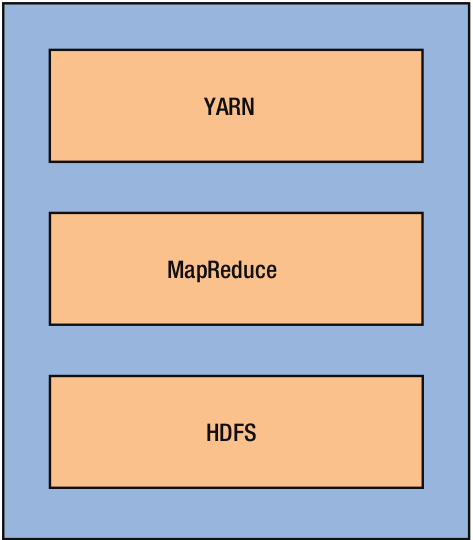
\includegraphics[width=0.4\textwidth]{hadoopCompo.png}
\caption{componenti principali di Hadooop}
\label{fig:hadoopComponets}
\end{figure} 
 
Uno dei fattori di successo di Hadoop è il basso costo. Hadoop è un sistema open-source che può essere eseguito su un cluster di commodity\footnote{hardware non dedicato di basso costo} hardware. Riesce cioè a garantire facilmente una scalabilità orizzontale aggiungendo al cluster, dei server poco costosi. Inoltre, riesce a garantire, via software la tolleranza ai guasti: assume che prima o poi vi saranno dei guasti e li gestisce in maniera trasparente. Uno sviluppatore software non dovrà preoccuparsi di gestire questi fault. Consente, cioè, di sviluppare applicazioni distribuite in maniera molto più semplice poiché viene sperata la logica di elaborazione dei dati dalla logica di distribuzione dei dati.
Hadoop è composto da tre componenti principali: un cluster mananger (YARN), un modello di computazione distribuito (Map-reduce) e un file system distribuito (HDFS)



 
 \subsubsection{Map Reduce}
 MapReduce \cite{Dean:2004:MSD:1251254.1251264} è il modello di computazione distribuita fornito da Hadoop. Mentre HDFS fornisce un file system distribuito per memorizzare grandi dataset, MapReduce fornisce un framework di computazione che consente di processare grandi dataset in parallelo attraverso un cluster di computer (nodi). Questo modello astrae la computazione distribuita fornendo dei costrutti ad alto livello che consentono di sviluppare facilmente applicazioni distribuite.
 Il framework MapReduce schedula in maniera automatica l'esecuzione di un applicazione su un insieme di macchine in un cluster, prendendosi carico  della gestione della comunicazione fra nodi, del bilanciamento del carico di esecuzione fra i nodi e dei possibili guasti dei nodi.
In questo modo, gli sviluppatori possono concentrarsi sulla logica di processing dei dati tralasciando questi dettagli.



 

Come suggerisce il nome stesso, questo modello si basa su due funzioni : \emph{map} e
\emph{reduce}. Tutti i carichi di lavoro in un applicazione MapReduce sono espressi implementando queste due funzioni. 


Tutti i carichi di lavoro in un applicazione MapReduce sono espressi implementando queste due funzioni.  
La funzione \emph{map} riceve in input una coppia chiave-valore e restituisce a sua volta una insieme di  coppie chiave valore intermedie. Il framework MapReduce esegue la funzione map per ogni coppia chiave valore presente nel dataset di input. L'output delle funzioni Map, è ordinato e raggruppato in base ai valori di chiave intermedi, e costituirà l'input della funzione Reduce. La funzione \emph{Reduce} aggrega i risultati della funzione map, in base al valore di chiave intermedio.
Fra la fase \emph{map} e la fase \emph{reduce}, vi è una fase intermedia detta \emph{shuffle} che consiste nel partizionare i dati in base al loro valore di chiave e indirizzarli al nodo reducer, ovvero il nodo su cui si dovrà eseguire la funzione \emph{reduce}.

I dati possono essere sia semi strutturati o non strutturati affatto, non è richiesto che i dati siano conformi ad uno schema rigido predefinito. L'unico requisito è che sia possibile esprimere il dataset in input come una serie di coppie chiave valore.
Il modello MapReduce ha rivoluzionato il modo di processare grandi datasets, offrendo un modello semplice che consente di scrivere programmi che possono essere eseguiti in parallelo su molte macchine. Grazie a questo, Map-Reduce consente di ottenere una scalabilità orizzontale: all'aumentare della dimensione dei dati è possibile aggiungere nuove macchine mantenendo quasi invariato il tempo di esecuzione.
\subsection{Apache Spark}
%Uno dei punti di forza del paradigma MapReduce, come abbiamo visto,  è quello di consentire all utente    di effettuare elaborazioni su larga scala senza che quest'ultimo di debba preoccupare di come distribuire la computazione sui vari nodi o come gestire i fallimenti di un nodo. Uno dei principiali svantaggi però di questo paradigma è dato dal fatto che non consente di implementare algoritmi che devono eseguire più iterazioni sugli stessi dati in maniera efficiente.
%Questa inefficienza è dovuta al fatto che i risultati intermedi della computazione vengono serializzati su filesystem.






Apache Spark \footnote{http://spark.apache.org/} è una framework open-source che consente di processare grandi dataset in maniera distribuita.
Spark può essere considerato come il successore del modello MapReduce di Hadoop, entrambi i framwork sono progettati per poter processare i big data.  Spark mantiene inalterata la scalabilità di MapReduce e la tolleranza ai guasti, e inoltre aggiunge nuove caratteristiche, offrendo inoltre ulteriori vantaggi rispetto a MapReduce. Primo fra questi è la velocità: Spark riesce a processare i dati riducendo  di molto i tempi di latenza (fino a 100 volte), poiché  consente ai nodi di processing di immagazzinare in memoria centrale i risultati intermedi, a differenza di MapReduce, dove invece erano serializzati sul file system.  



La velocità può essere talvolta un fattore determinante. Impiegare troppo tempo per processare i dati, rallenta tutto il processo decisionale riducendo il valore stesso dei dati.
La principale astrazione fornita da SPARK sono i \textbf{R}esilent \textbf{D}istributed \textbf{D}ataset (RDD) \cite{Zaharia:2012:RDD:2228298.2228301}, che essenzialmente sono una collezione immutabile e distribuita di oggetti. Questi oggetti sono, suddivisi in più partizioni che  generalmente sono distribuite su più nodi.

Questa astrazione permette agli sviluppatori di materializzare i risultati intermedi della computazione nella memoria dei vari nodi di processing. Ciò significa che i prossimi step che vogliono riconsultare questi dati, non li dovranno rielaborare o ricaricare da
disco. Per tale ragione, Spark  si presta bene per eseguire in parallelo sia algoritmi altamente iterativi che richiedono di scansionare un dataset di input
più volte, come gli algoritmi di machine-learning come   PageRank, K-means clustering, e logistic regression.




Architetturalmente, Spark è progettato per essere altamente accessibile: offre API per Python, Java, Scala, SQL e R. Inoltre si integra alla perfezione con strumenti di Big Data quali Hadoop (e strumenti che dipendono da esso come HBase, Hive, etc.) e Cassandra.




 
\begin{figure}[htbp]
    \makebox[\textwidth]{
        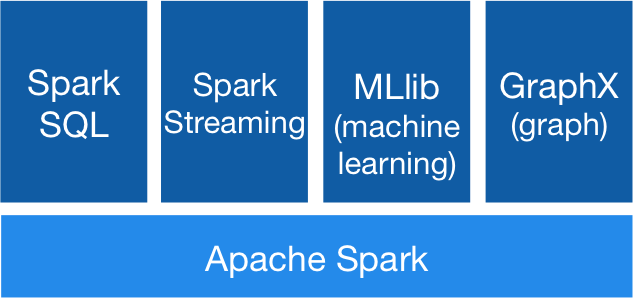
\includegraphics[width=0.7\textwidth]{spark-stack.png}
    }
    \caption{Stack applicativo Apache Spark}
    \label{fig:sparkstack}
\end{figure}




La figura \ref{fig:sparkstack} mostra le principali componenti di Apache Spark:
\begin{itemize}
\item \textbf{Spark Core}: contiene le funzionalità base di Spark fra cui l'astrazione sulla quale si basa l'intero ambiente, i \textit{resilient distributed dataset} (RDD).
\item \textbf{Spark SQL}: contiene le componenti per elaborare e manipolare dati strutturati. Permette l'interrogazione (tramite SQL) di dabatase relazionali, JSON, HIVE (mediante lo Hive Query Language) e file Parquet. 
\item \textbf{Spark Streaming}: componente che permette l'elaborazione di stream di dati.
\item \textbf{MLLib}: contiene algoritmi di Machine Learning per vari tipi di task quali classificazione, regressione, clustering, collaborative filtering, frequent pattern mining, dimensionality reduction, feature extraction e statistica di base.
\item \textbf{GraphX}: libreria per la manipolazione ed estrazione di conoscenza in grafi.
\end{itemize}

\subsection{Resilent Distribuited Dataset}
Formalmente un RDD è una collezione di oggetti immutabile e partizionata.
Questi RDD possono essere creati in due modi: o a partire da dati in un sistema di memorizzazione stabile\footnote{per stabile si intende fault-tolerant} (HDFS, Hive, Cassandra, ) o a partire da altri RDD, mediante un insieme di operatori messi a disposizione dal framework come map, reduce, groupByKey etc. 
Questo tipo di  operazioni, che creano RDD, sono dette \emph{trasformazioni}. Spark offre due tipologie di operazioni:
\begin{itemize}
\item \textbf{Trasformazioni} operazioni che producono nuovi RDD a partire da un rdd come \emph{map,filter,join}
\item \textbf{Azioni} queste operazioni invece restituiscono un valore all'applicazione o esportano i dati presenti nell'RDD in un sistema di memorizzazione.
Alcuni esempi di \emph{action} sono \emph{count} (che restituisce il numero di elementi nel dataset), \emph{collect} (che restituisce tutti gli elementi stessi, e \emph{save} che  memorizza il dataset su un dispositivo di memorizzazione.
\end{itemize}
Bisogna sottolineare che in Spark gli RDD  sono valutati in maniera pigra \emph{(lazy evaluated)} ovvero sono computati solo la prima volta che sono utilizzati in una azione.
 

I programmatori possono controllare inoltre due aspetti fondamentali di un RDD: 
\begin{inlinelist}
  \item caching,
  \item partitioning.
\end{inlinelist}
 Un utente, se  ha intenzione di riutilizzare i dati in più step, può richiedere che un RDD sia conservato in memoria cache, in tal caso verranno memorizzate nella memoria dei nodi di processing le partizioni dell'RDD.  Se  non vi è memoria sufficiente per memorizzare una qualche partizione dell'RDD, questa verrà scritta su disco.
Se si ha intenzione di riutilizzare i dati in più step, l'utente può decidere di memorizzarlo nella cache dei nodi di processing, in modo tale che non venga  rielaborato. 

 

Inoltre è possibile che gli elementi di un RDD siano partizionati lungo le macchine nel cluster, in base al valore chiave di ciascun record. Ad esempio è possibile richiedere che due RDD siano (hash) partizionati nello stesso modo, facendo sì che i record con la stessa chiave siano sulla medesima macchina, in questo modo operazioni come un join fra due rdd 
saranno molto più veloci poiché i dati non dovranno essere spostati lungo la rete.
 
  
  
A differenza di altri approcci di distribuzione dei dati che replicano i dati su più nodi, in spark per ogni RDD viene memorizzato il suo \emph{lineage} ovvero la sequenza di trasformazioni che lo ha prodotto, a partire da un altro RDD. In tal modo SPARK nel caso vi sia un failure, può rielaborare un RDD in maniera del tutto trasparente.
 
Gli RDD posssono contenere qualsiasi tipo di oggetti \footnote{poiche Spark è eseguito su una JVM, questi elementi sono oggetti JAVA} , che sono suddivisi in
partizioni in maniera automatica lungo il cluster. Questi oggetti una volta
creati, sono immutabili e possono essere creati solo tramite gli operatori
di Spark.
Ad esempio dato un RDD di coppie \texttt{(visitID,URL)} contenente le visiste di
alcuni siti internet, è possibile ottenere un nuovo RDD contenente per ciascun
sito il numero di visite ricevute \texttt{(URL,count)}, applicando l’operatore map
trasformando ogni coppia iniziale \texttt{(visitID,URL)} in una coppia \texttt{(URL,1)} e
poi applicando l'operatore \emph{reduce} per ottenere il numero di visite per ciascun sito.

In seguito è mostrato un frammento di codice in scala per ottenere tale
risultato:\\
\texttt{visits=spark.hadoopFile("hdfs://....")}\\
\texttt{val counts=visit.map(v=>(v.url,1)).reduceByKey( + )}\\


\begin{figure}[htbp]
    \makebox[\textwidth]{
        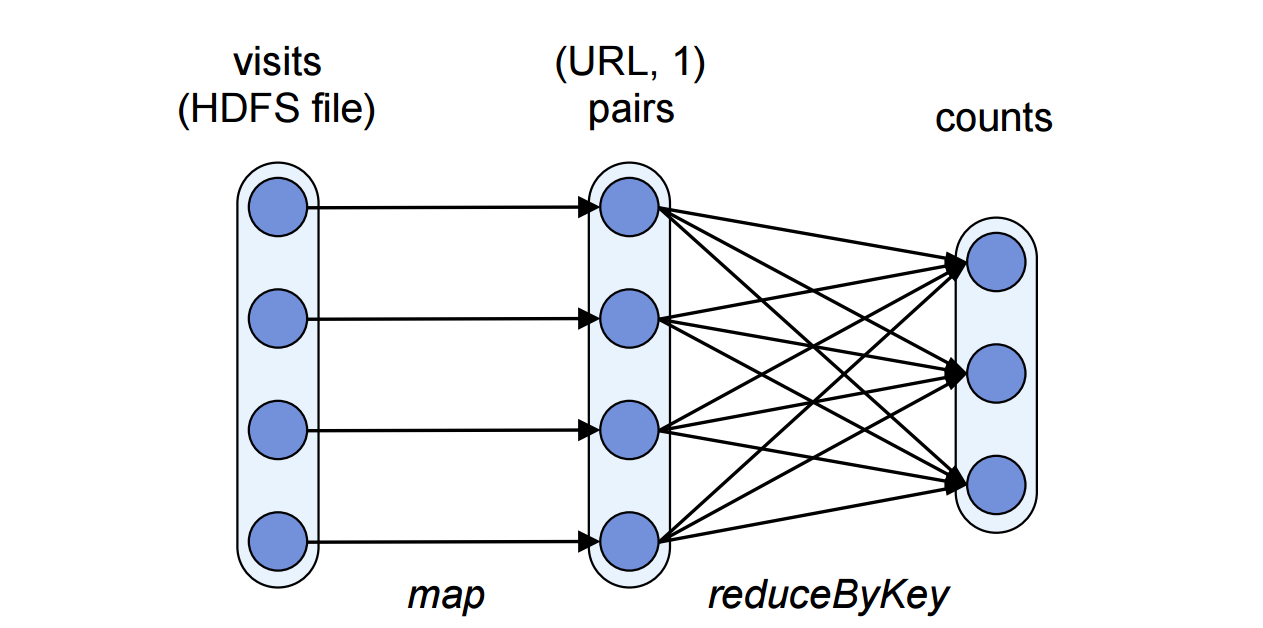
\includegraphics[width=0.7\textwidth]{sparkRDDexample.png}
    }
    \caption{Esempio di lineage Graph: Gli ovali rappresentano gli RDD, i pallini le partizioni}
    \label{fig:lineageRDD}
\end{figure}

La figura \ref{fig:lineageRDD} mostra il lineage-graph degli rdd in esempio. Se
viene persa una partizione dell'RDD \texttt{(URL,1)} sarà possibile ricalcolarla
rieseguendo l'operatore map, sulla corrispondente partizione.

\begin{figure}[h]
\centering
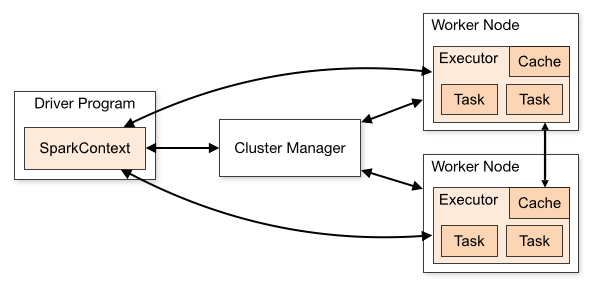
\includegraphics[width=0.8\textwidth]{cluster-ov.png}
\caption{componenti Di Un Cluster in Spark}
\label{fig:sparkClusterComponents}
\end{figure} 

 Al fine di utilizzare le funzionalità di Spark, uno sviluppatore deve fornire un programma \emph{driver} che si connette ad un cluster di nodi \emph{worker} su cui verranno eseguiti i processi \emph{Executor}  come mostrato in figura \ref{fig:sparkClusterComponents}.
 Nel programma driver saranno definiti uno o più RDD che saranno valutati solo alla prima occorrenza di \emph{action} su di essi. Su ciascun nodo worker sarà possibile memorizzare in memoria RAM le partizioni degli RDD, che sono rappresentate come oggetti JAVA.
Gli   stessi RDD sono rappresentati come  oggetti tipizzati staticamente con un parametro di tipo ,ad esempio ,
\texttt{RDD[Int]} rappresenta un dataset di interi.  

In particolare   ogni RDD è descritto da  
\begin{inlinelist}
  \item un insieme di partizioni (componenti atomiche di un dataset);
  \item un insieme di dipendenze (che definiscono il suo \emph{lineage};
  \item dei metatdati riguardanti lo schema di partizionamento e il posizionamento dei dati lungo il cluster.
\end{inlinelist}
Ad esempio, un RDD generato a partire da un file HDFS, avrà una partizione  in corrispondenza di ciascun blocco del file, e i saprà su quale nodo è memorizzato ciascun blocco.
Sebbene in Spark  cerca di eseguire il codice il più vicino possibile ai dati, per evitare spostamenti dei dati lungo la rete (\emph{shuffle}, talvolta questi spostamenti sono inevitabili.
Le dipendenze in Spark  sono categorizzate in
\begin{itemize}
\item \textbf{narrow}  
ogni partizione del RDD padre è usata al più da una partizione del RDD figlio \footnote{un RDD generato a partire da un altro RDD attraverso una trasformazione}. Ciò significa che le partizioni possono essere calcolate localmente su ogni nodo worker, senza generare shuffle dei dati. (e.g: map(), filter()..) 
 \item \textbf{wide}  dove ogni partizione del figlio può dipendere da ciascuna partizione del nodo padre. Ciò implica che i dati saranno inviati lungo la rete attraverso un'operazione di shuffle dei dati.(e.g:reduceByKey(), join(), groupByKey()), a meno chè i parent RDD siano stati partizionati in base al valore di chiave.(hash-partitioned)
\end{itemize}

   \begin{figure}[h]
\centering
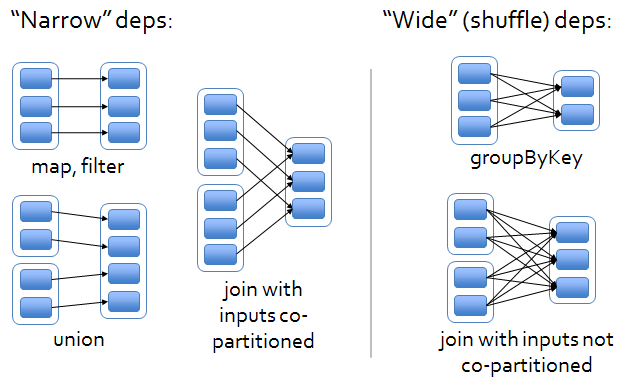
\includegraphics[width=1.0\textwidth]{dipendenze.png}
\caption{Esempi di dipendenze wide e narrow. ogni contenitore rappresenta un RDD, i rettangoli le partizioni}
\label{fig:exPlanSPark}
\end{figure} 
Questa distinzione è fondamentale in quanto le \emph{narrow} consetono a Spark di raggruppare le computazioni sui nodi worker.
Mentre nel caso di dipendenze di tipo wide è necessario che tutte le partizioni del parent rdd siano state elaborate su tutti i nodi, e verranno inviate lungo la rete attraverso delle operazioni di shuffle.
Inoltre per le dipendenze di tipo \emph{narrow} è molto più semplice rielaborare dei dati in caso di failure di un nodo, poiché verranno ricalcolate le sole partizioni del nodo dove è avvenuto il guasto; al contrario nel caso di \emph{wide-dependencies} bisognerà rielaborare tutte le partizioni.
Lo scheduler dei task di Spark si avvale di queste distinzioni per ottimizzare la computazione.
Quando viene invocata una \emph{action} su un RDD, lo scheduler esamina il grafo delle dipendenze del RDD in questione per costruire un piano di esecuzione espresso come un grafo diretto aciclico di stage. Lo scheduler cerca di accorpare il maggior numero possibile di  dipendenze di tipo narrow in ciascuno stage.
Ai bordi di ciascuno stage, come è possibile osservare in figura \ref{fig:exPlanSPark} vengono postele operazioni di \emph{shuffle} richieste per le dipendenze di tipo wide, o quelle partizioni che sono state poste in memoria cache. Lo scheduler cerca di allocare  \emph{task} seguendo il principio della \lq\lq località dei dati\rq\rq in modo tale ad minimizzare la comunicazione fra i vari nodi.


 
 
    \begin{figure}[h]
\centering
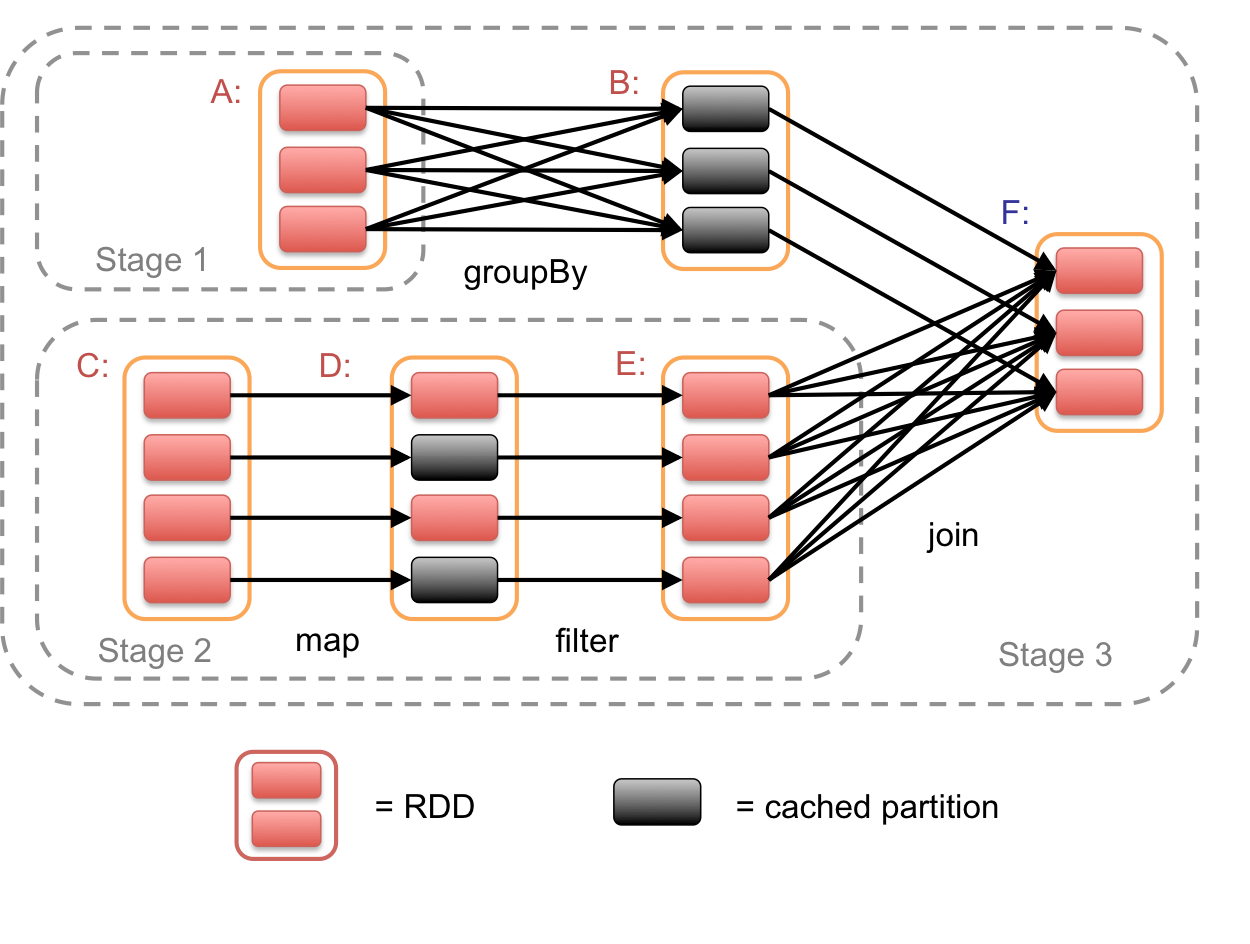
\includegraphics[width=1.0\textwidth]{executionPlan.png}
\caption{Esempio di un piano di esecuzione}
\label{fig:sparkDependencies}
\end{figure} 

 

\section{DBpedia}
Wikipedia \footnote{https://en.wikipedia.org/} è divenuta una delle maggiori risorse di conoscenza disponibili nel web, ed è manutenuta da migliaia di utenti (collaboratori). Gli articoli Wikipedia sebbene composti prevalentemente da testo, contengono informazioni semi-strutturate come: template infobox , informazioni sulla categorizzazione dell'articolo, immagini, geo-coordinate e link sia verso altre pagine web sia verso altre pagine wikipedia.
Gli infobox sono tabelle di coppie attributo valore, che mostrano i dati più rilevanti di ciascuna pagina wikipedia. Il progetto DBpedia \cite{Bizer:2009:DCP:1640541.1640848} estrae dati strutturati da wikipedia tramite un extraction framweork open source e li unisce in una base di conoscenza multi dominio e multi lingua. Per ogni pagina presente in wikipedia, viene associato un \emph{Uniform Resource Identifier (URI)} in DBpedia per identificare un'entità o un concetto descritto dalla corrispondente pagina Wikipedia della versione inglese. Durante il processo di trasformazione, i dati semi-strutturati come i campi infobox,categorie, pagelinks sono convertiti in triple RDF e aggiunte alla base di conoscenza come proprietà dell'entità identificata dall URI.  Per rendere omogenea la descrizione delle informazioni, è stata sviluppata un ontologia e sono state definite le corrispondenze fra le proprietà presenti negli infobox e l'ontologia.
L'ontologia DBpedia consisite di 320 classi e descritte da 1650 proprietà. Le classi organizzate mediante una gerarchia sussuntiva dove \emph{owl:Thing} è la classe più generale. Poiché Il sistema di Wikipedia infobox si è evoluto in maniera decentrata, talvolta accade ad esempio che si usino diversi template per la stessa tipologia di entità (class) o si usino nomi diversi per descrive lo stesso attributo (es placeOfBirth o birthPlace). 
 L'allineamento tra i template infobox e l'ontologia a causa di queste eterogeneità presenti nella nomenclatura, non è quindi completamente automatico, ma si basa anche su mapping definiti manualmente, forniti dalla comunità di DBpedia. Ad esempio ‘date of birth’ and ‘birth
date’ sono entrambi mappati con la proprietà birthDate. 
 
 La base di conoscenza DBpedia è disponibile sul web sotto GNU Free Documentation, e può essere consultata mediante varie modalità :
\begin{itemize}
\item \textbf{Linked Data}: linked data è la metodologia di pubblicazione  dei dati RDF nel web, che utilizza gli URI http come identificativo delle risorse e il protocollo HTTP per ritrovare al descrizione rdf delle risorse. Quando si accedere ad un URI di una risorsa DBPedia mediante un semantic web agent si ottiene la descrizione rdf della risorsa mentre se si utilizza un semplice web-browser si otterrà una vista html della descrizione.
\item \textbf{Sparql Endpoint } \'E fornito un endopoint mediante il quale si può interrogare la base di conoscenza tramite il protocollo SPARQL.
\item \textbf{RDF dumps} la base di conoscenza è stata suddivisa in varie parti in base agli rdf-predicate 
\end{itemize}